% !TeX root=main.tex
\chapter{入出力制御回路}

%%%%%%%%%%%%%%%%%%%%%%%%%%%%%%%%%%%%%%%%%%%%%%%%%%%%%%%%%%%%%%%%%%%%%%%%%%%%%%
\section{ベース設計の内部構造}

図\ref{fig:iodetail}に,より詳細なベース設計のブロック図を示します.ソースコード
は,パッケージの DRFront/BaseDesign\_RC フォルダに置かれており,図中の青字は回路名
またはソースコードのファイル名を示しています.青色白抜きで示している DR\_TOP が
ユーザ回路で,それ以外が入出力制御回路です.

\begin{figure}[ht]
 \centering
 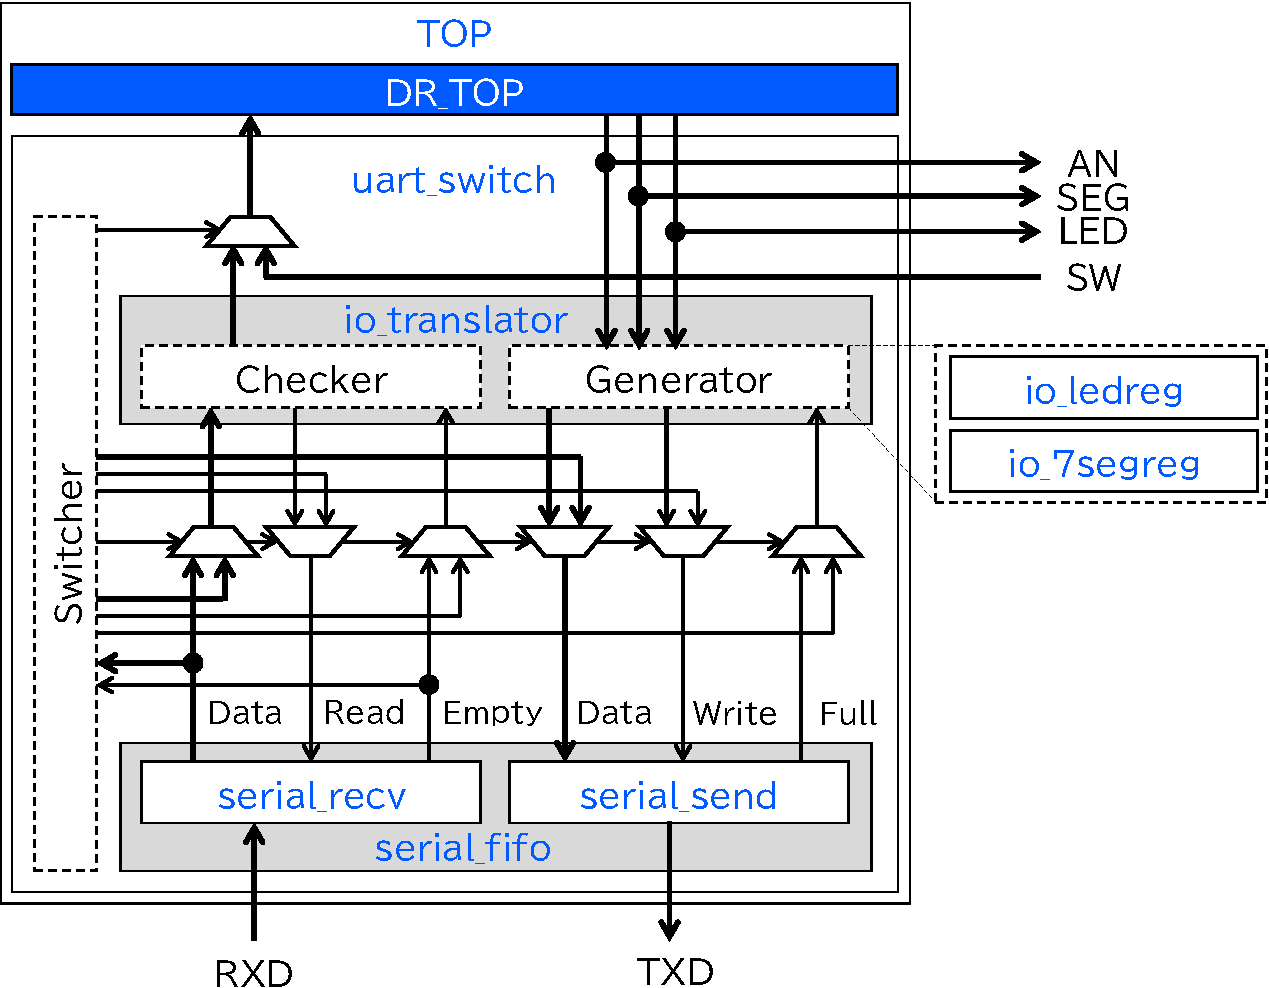
\includegraphics[width=110truemm]{figs/iodetail.pdf}
 \caption{ベース設計の内部構造.}
 \label{fig:iodetail}
\end{figure}

入出力制御回路には3つの主要な回路が組み込まれています.1つは UART コントローラ
(serial\_fifo),1つは I/O トランスレータ(io\_translator),もう1つはスイッチャー
回路(uart\_switch の内部回路)です.UART コントローラは,FPGA ボードの USB-UART
入出力に対するシンプルな FIFO インタフェースを提供します.I/O トランスレータは,
出力の生成回路(Generator)部分と入力のチェック回路(Checker)部分とに分かれて
います.

出力の生成回路部分では,コントローラボードが知っているであろう LED 出力の値を保持し,
現在のユーザ回路の出力と比較します.もし差異があれば,その中から1つを選択して,
コマンド文字列を生成するとともに,保持している LED 出力の値を更新します.

生成回路部分ではまた,出力のサンプリングも行っています.この目的は3つです.
第1の目的は,コマンドの生成される頻度を減らすことです.そのために,7セグメント
LED では 100 Hz で,通常の LED では 500 Hz で,それぞれ出力をサンプリングしています.
第2の目的は,通常ダイナミック点灯により制御される7セグメント LED の表示を安定
させるためです.そのために,サンプラーは7セグメント LED がどのように見えるかを
判定します.見た目が変わらない限りは生成回路部分からコマンドが送信されることは
ありません.第3の目的は,PWM 出力をおおまかに再現することです.ユーザが LED に
PWM 信号を与えていた場合,その周期がサンプリング周期と一致してしまうと,意図した
出力がコントローラボード上に得られないかもしれません.これを防ぐため,通常の LED
用のサンプラーは,単なるサンプリングではなく `1' が出力されていた割合をチェック
します.これが周期的に変化するしきい値よりも大きかった場合に,その LED 出力は `1'
であると判定します.

入力のチェック回路部分では,現在のスイッチ入力の値を保持し,コマンド文字列を待ちます.
スイッチをオン・オフするコマンド(`U' または 'u')を受信したら,対応するスイッチ
入力の値を `1' または `0' に変更します.

スイッチャー回路は,リセット直後は Connector アプリからの応答要求(``VX'')が送信
されるまで待機します.またこの間は,ボードのスイッチ入力をそのままユーザ回路へと
渡すとともに,I/O トランスレータからの信号をブロックします.これにより,FPGA
ボードが単体で動作している場合には,あたかもユーザ回路だけが動作しているかの
ように見えます.応答要求を受信したら,I/O トランスレータからの信号のブロックを
解除します.

%%%%%%%%%%%%%%%%%%%%%%%%%%%%%%%%%%%%%%%
\section{ベース設計の論理合成}

ベース設計の論理合成は,AMD FPGA の動的部分再構成(DFX)機能を使って行うため,
通常の論理合成とは方法が異なります.本節では,ソースコードからベース設計を論理合成
する手順を説明します.
なお,ソースコードの一部は対象とする FPGA ボードによって異なります.以降の説明では,
これを〈ボード名〉と表記します.ボード名は,Nexys,Arty,CMod のいずれかです.

\begin{enumerate}
 \item プロジェクトを新規作成し,ユーザ回路として空の回路を指定して,回路全体を
 論理合成します.設計のソースとして dr\_top.vhdl と 〈ボード名〉/dr\_base.vhdl
 \textbf{以外の}すべての VHDL ファイル,制約ファイルとして
 〈ボード名〉/〈ボード名〉.xdc を指定します.ロジックアナライザ(ILA)の IP コア
 設定として 〈ボード名〉/ila\_0.xci も設計のソースに追加します.
 \item 論理合成が終了したら,Open Synthesized Design で合成後の設計を開き,
 「File」→「Checkpoint」→「Write」でチェックポイントを保存します.保存したチェック
 ポイントファイルを,以後 step\_1.dcp とします.合成後の設計を開いた際に警告
 (Project 1-486)が表示されますが,無視して構いません.
 \item 別のプロジェクトを新規作成し,dr\_top.vhdl と 〈ボード名〉/dr\_base.vhdl
 を使って,デフォルトのユーザ回路を論理合成します.このとき,SYNTHESIS を右クリック
 して Synthesis settings を開き,More Options の欄に\texttt{-mode out\_of\_context}
 と入力します.これにより,不要な I/O バッファの挿入を抑止できます.
 \item 論理合成が終了したら,ステップ2と同様にチェックポイントを保存します.
 保存したチェックポイントファイルを,以後 step\_3.dcp とします.
 \item 「File」→「Checkpoint」→「Open」で step\_1.dcp を開きます.警告
 (Project 1-486)は無視して構いません.
 \item Tcl Console に以下のコマンドを打ち込み,ベース設計にデフォルトのユーザ回路を
 組み込みます.ただし,\texttt{/PATH/TO/CHECKPOINT} はチェックポイントを保存した
 フォルダのパス名とします.
\begin{verbatim}
    set_property HD.RECONFIGURABLE true [get_cells DR]
    cd /PATH/TO/CHECKPOINT
    read_checkpoint -cell [get_cells DR] step_3.dcp
\end{verbatim}
 \item ユーザ回路の配置される範囲(Pblock)を指定します.Vivado の画面右上 Device
 タブで,Draw Pblock のボタン(P+と書かれたアイコン)をクリックして,スライスや
 DSP,BRAM を含む適当な範囲を囲みます.
 \item 指定した Pblock の範囲に問題がないかチェックします.「Reports」→「Report DRC」
 を選択し,Rules で Dynamic Function Exchange にのみチェックを入れた状態で,DRC を
 実行します.もし DRC に失敗したら,エラーメッセージに従って Pblock の範囲を修正して,
 やり直してください.
 \item Tcl Console に以下のコマンドを打ち込み,作成した Pblock の範囲の設定を保存
 します.
\begin{verbatim}
    write_xdc -force PBLOCK.xdc
\end{verbatim}
 2回目以降は Pblock の範囲指定は \texttt{read\_xdc PBLOCK.xdc} で行えます.
 \item Tcl Console に以下のコマンドを打ち込み,実装とビットストリームファイルの作成
 を行います.
\begin{verbatim}
    opt_design
    place_design
    route_design
    write_bitstream -force -bin_file base.bit
    write_debug_probes -force base.ltx
\end{verbatim}
 \item Tcl Console に以下のコマンドを打ち込み,ユーザ回路を空の回路に戻した状態で
 チェックポイントを作成します.ここで作成したチェックポイントファイルを DRFront で
 使用します.
\begin{verbatim}
    update_design -cell DR -black_box
    lock_design -level routing
    write_checkpoint -force base.dcp
\end{verbatim}
\end{enumerate}

%%%%%%%%%%%%%%%%%%%%%%%%%%%%%%%%%%%%%%%%%%%%%%%%%%%%%%%%%%%%%%%%%%%%%%%%%%%%%%